\chapter{Venerdì 12/03/2021, Lunedì 15/03/2021 e Martedì 16/03/2021}

\section{Programmazione mista: funzioni}
Per scrivere funzioni in C++ e chiamarle da Assembler, e viceversa, dobbiamo tener conto di una serie di regole, in particolare dobbiamosapere come avviene il passaggio dei parametri (in ingresso e in uscita) e dove vengono poste le variabili locali. La soluzione adottata è sofisticata (non è la prima cosa che viene in mente a una funzione).

\paragraph{Cosa serve a una funzione?}
Una qualunque funzione avrà bisogno di:
\begin{itemize}
	\item uno spazio per i parametri in ingresso, in uscita, e i risultati intermedi;
	\item uno spazio per le istruzioni.
\end{itemize}
%La cosa può essere immaginata in modo molto elementare
%\begin{center}
%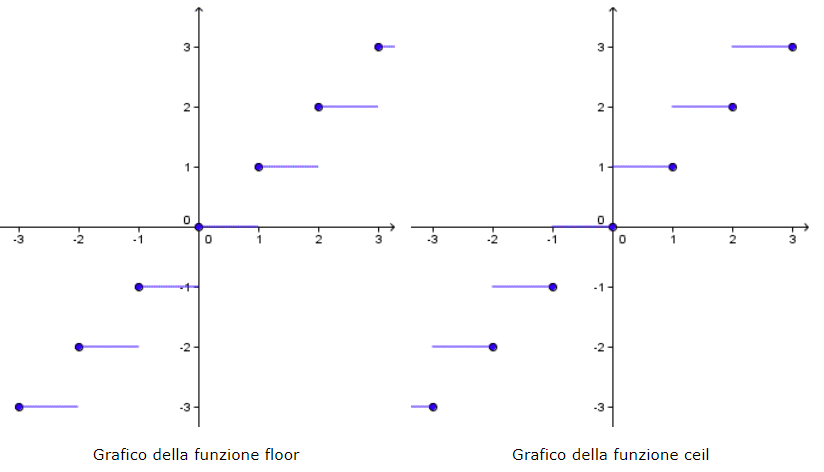
\includegraphics[scale=0.90]{img/19.PNG}
%\end{center} 
\paragraph{Preallocazione?} La preallocazione dello spazio per parametri e risultati intermedi è svantaggiosa: 
\begin{itemize}
	\item si consuma troppo spazio;
	\item non è possibile fare chiamate ricorsive della stessa funzione;
	\item non è possibile condividere lo stesso codice in simultanea a più flussi.
\end{itemize}

\paragraph{Quindi?} L'idea è di mettere questi parametri su una pila, ponendo il cosiddetto \emph{record di attivazione}.
\clearpage 
\subsection{Record di attivazione}
Ogni volta che si chiama una funzione si alloca nella pila il cosiddetto \emph{record di attivazione della funzione}, che contiene variabili locali, parametri, e l'indirizzo di ritorno.
\begin{center}
	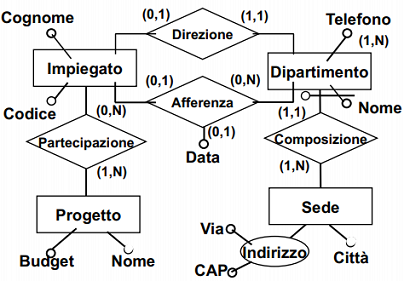
\includegraphics[scale=0.59]{img/20.PNG}
\end{center} 
L'indirizzo di ritorno è cosa già vista: lo inserisco in pila con la CALL e lo rimuovo con la RET. La funzione accede ai vari campi del record di attivazione in modo indiretto. Dobbiamo tener conto che l'indirizzo di questi elementi non è fisso, considerando che potrei avere altre chiamate ricorsive prima di quella attuale che stiamo considerando. Una soluzione è calcolare l'offset rispetto al registro rsp
\begin{verbatim}
	offset(%rsp)
\end{verbatim}
rimane il fatto che se durante l'esecuzione del programma alteriamo la RSP allora gli offset dovranno essere ricalcolati. I processori moderni lo sanno fare senza grossi problemi.
\paragraph{Architettura Intel} Nell'architettura Intel si tende a usare un registro esplicito che punti al record di attivazione senza usare rsp. Introduciamo il registro RBP (\emph{Register Base Pointer}): per tutta la durata di esecuzione della funzione il valore di questo registro è costante e punta a un punto preciso del record di attivazione, subito sopra l'indirizzo di ritorno. Ad ogni chiamata di funzione viene memorizzato il valore precedente di rbp mediante PUSH.
\begin{verbatim}
	PUSH %rbp <--- salvo il valore vecchio 
	MOV %rsp, %rbp <--- aggiorno il contenuto del registro
\end{verbatim}
alla fine dell'esecuzione, se RSP è stato riportato al suo valore iniziale, diremo
\begin{verbatim}
	POP %rbp <--- recupero il valore vecchio 
	RET
\end{verbatim}
Nel caso in cui ciò non avvenga basta eseguire un'istruzione MOV (non ne avremo bisogno, basta rispettare le regole sull'uso di PUSH e POP). Per terminare il record di attivazione basta riservare spazio per i parametri e le variabili locali. Questo è semplice
\begin{verbatim}
	SUB $spazio, %rsp
\end{verbatim}
Sposto rsp in modo che successive push o chiamate di funzione proseguano oltre senza toccare questo spazio. La struttura del record di attivazione (relativamente a parametri e variabili locali) è flessibile: il suo contenuto interessa solo alla funzione.

\subsubsection{Passaggio di parametri in ingresso}  Altra cosa che deve fare il chiamante è passare i parametri. Chiaramente non può scriverli nel record di attivazione direttamente, visto che si muoverà prima che venga riservata l'area di memoria. Osserviamo le differenze tra le due architetture
\begin{itemize}
	\item \textbf{Architettura a 32bit}: i parametri vengono posti nella pila prima di eseguire la call
	\begin{framed}
		\item \textbf{Architettura a 64bit}: sfruttando il numero più alto di registri si passa i parametri direttamente con questi. Possiamo avere varie situazioni
		\begin{itemize}
			\item Pongo i parametri nei registri e li mantengo qua senza spostarli nell'aria di memoria
			\item Pongo i parametri nei registri e li sposto nell'area di memoria dedicata ai parametri e alle variabili locali. In quali occasioni sono costretto a fare così?
			\begin{itemize}
				\item Quando devo chiamare altre funzioni, oppure
				\item quando devo utilizzare istruzioni che ricorrono per forza a certi registri (moltiplicazione, divisione, istruzioni per le stringhe)
			\end{itemize}
		\end{itemize}
		se la funzione ha più di 6 argomenti si adotta, per gli argomenti in eccesso, la strategia vista per l'architettura a 32bit. Si usano i seguenti registri, nell'ordine seguente...
		\begin{multicols}{3}
			\begin{enumerate}
				\item \%RDI
				\item \%RSI
				\item \%RDX
				\item \%RCX
				\item \%R8
				\item \%R9
			\end{enumerate}
		\end{multicols}
		(D,S,D,C,8,9) Abbiamo già indicato questi registri come registri scratch: quali registri scratch possiamo usare dipenderà dalle situazioni.
	\end{framed}
\end{itemize}

\paragraph{Osservazione} Argomenti diversi usano registri diversi. Se io ho, per esempio... 
\begin{verbatim}
	f(char c, char b);
\end{verbatim}
non posso metterli nello stesso registro: c va in rdi, b in rsi.\\

\noindent \textbf{Esempio di situazione in cui i parametri non vengono mantenuti nei registri}

\begin{multicols}{3}
	\begin{verbatim}
		struct s {
			int i[4];
		}
	\end{verbatim}
	\begin{verbatim}
		int f(s x) {
			g(&x);
		}
	\end{verbatim}
	\begin{verbatim}
		g(s* p) {
			...
		}
	\end{verbatim}
\end{multicols}
\noindent Non possiamo tenere il parametro solo nei registri, visto che questi non hanno indirizzo. Devo spostare il contenuto della struttura in memoria, a quel punto, avrò qualcosa che potrò puntare a partire dalla mia funzione.

\subsubsection{Parametro in uscita} La funzione termina: dove pongo il risultato? Abbiamo due possibilità
\begin{verbatim}
	%RAX
	%RDX_%RAX <--- (In caso di estensione)
\end{verbatim} 
O utilizzo solo il registro rax, oppure utilizzo anche il registro rdx (ponendo in rdx la parte più significativa di ciò che voglio restituire.\\
\scriptsize

\noindent \textbf{Hey} Questa cosa dovrebbe accenderci la lampadina.
\begin{verbatim}
	XOR %EAX, %EAX ----------> return 0;
\end{verbatim}
Stea ci ha detto che per convenzione si pone questa istruzione al termine del programma. Adesso capiamo perché!
\normalsize
\paragraph{Osservazione sulla dimensione dei parametri in ingresso e in uscita} 
\begin{itemize}
	\item Se io passo in ingresso una struttura e questa è grande al più 16 byte, questa dovrà essere passata con uno o due registri (la prima riga va in rdi, la seconda in rsi). 
	\item Se la struttura in ingresso è più grande di 16 byte la cosa è più complicata, ne riparleremo più avanti. 
\end{itemize}
Stesso ragionamento vale nella restituzione (con i registri citati prima).




\subsection{Esempio di struttura passata come parametro in ingresso}
\begin{center}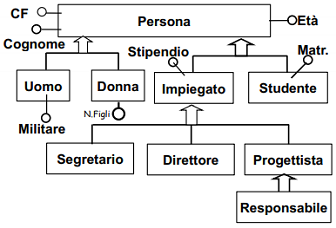
\includegraphics[scale=0.85]{img/22.PNG}\end{center}
\begin{verbatim}
	struct s {
		int i[4];
	}
	int f(s x) {
		int sum = 0;
		for(int j = 0; j < 4; j++)
		sum += x.i[j];
		return sum;
	}
\end{verbatim}
Il contenuto dell'elemento s sarà diviso tra rdi ed rsi. La cosa ottenuta non è molto comoda:
\begin{itemize}
	\item i[0] e i[2] possono essere recuperati, rispettivamente, coi registri EDI ed ESI
	\item ma gli altri due elementi?
\end{itemize}
L'unica cosa possibile è shiftare.


\subsection{Esercizio dalle diapositive del prof.Frosini}
\begingroup
\small
\subsubsection{Passaggio di parametri per valore (pag.35)}
\begin{framed}
	\noindent \textbf{Codice c++}
	\begin{multicols}{2}
		\begin{verbatim}
			// programma sommmaintGlob, file es1a.cpp
			#include"servi.cpp"
			extern "C" int elab1(int n, int m);
			int alfa, beta;
			int main() { 
				int ris;
				alfa = leggiint(); 
				beta = leggiint();
				ris = elab1(alfa, beta);
				scriviint(ris); 
				nuovalinea();
				return 0;
			};
			
			// programma sommmaintGlob, file es1b.cpp
			extern "C" int elab1(int n1, int n2) { 
				int i, j;
				i = n1+n2;
				j = n1-n2;
				
				return i*j;
			};
		\end{verbatim}
\end{multicols}\end{framed}
\noindent \textbf{Funzione \emph{elab1} in Assembler}
\begin{multicols}{2}
	\begin{verbatim}
		.global elab1
		elab1:
		push %rbp
		mov %rsp, %rbp
		sub $16, %rsp
		
		mov %edi, -8(%rbp)
		mov %esi, -4(%rbp)
		
		# i = n1 + n2
		mov %edi, -16(%rbp)
		add %esi, -16(%rbp)
		
		# j = n1 - n2
		mov %edi, %eax
		sub %esi, %eax
		mov %eax, -12(%rbp)
		
		# return i*j
		imull -16(%rbp), %eax
		
		leave   
		ret
	\end{verbatim}
\end{multicols}

\begin{itemize}
	\item Per prima cosa gestiamo il registro RBP 
	\begin{verbatim}
		push %rbp
		mov %rsp, %rbp
	\end{verbatim}
	salviamo in pila il valore vecchio e aggiorniamo il registro con l'RSP attuale.
	\item Riserviamo lo spazio per le variabili locali e i parametri di ingresso
	\begin{verbatim}
		sub $16, %rsp
	\end{verbatim}
	Riempiamo lo spazio appena allocato:
	\begin{center}
		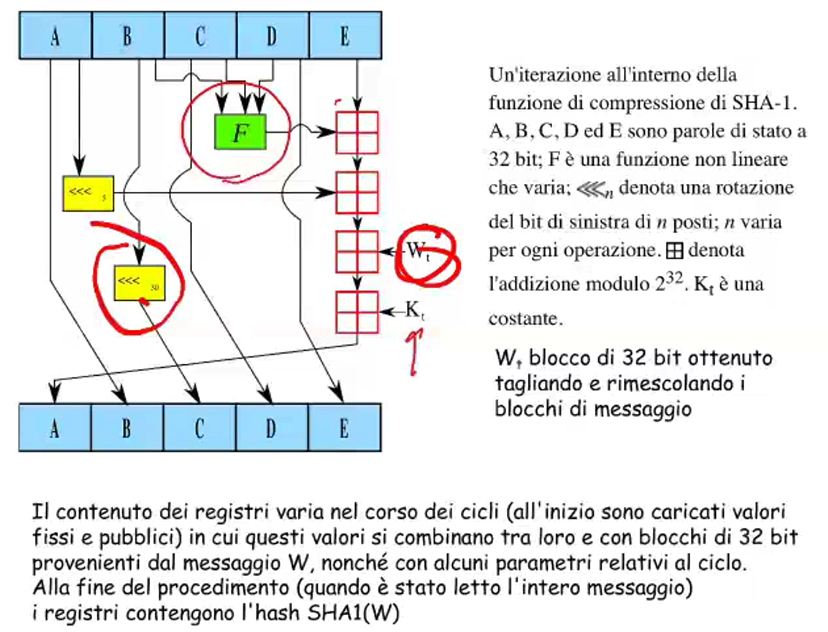
\includegraphics[scale=.85]{img/33.PNG}
	\end{center} 
	nell'indirizzamento si deve fare riferimento ad RBP (in questo caso potrei fare riferimento anche ad RSP, ma in generale è rischioso farlo). I registri source sono quelli che abbiamo citato, utilizzati nell'ordine indicato (in questo caso RDI ed RSI). 
	\begin{verbatim}
		mov %edi, -8(%rbp)
		mov %esi, -4(%rbp)
	\end{verbatim}
	Abbiamo due \emph{int} in ingresso, dunque bastano le parti meno significative a 32 bit.
	\begin{framed}
		\item \textbf{Domanda}. Come capisco quale sia il destinatario di queste istruzioni? Mi basta sommare il numero a destra con quello in alto. Riguardo la seconda MOV la tentazione potrebbe essere scrivere quanto segue
		\begin{verbatim}
			mov %esi, -12(%rbp)
		\end{verbatim}
		Ricordarsi che siamo in una pila, dunque andiamo indietro e non in avanti. 
		\begin{center}
			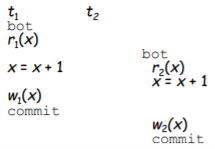
\includegraphics[scale=.65]{img/153.PNG}
		\end{center} 
	\end{framed}
	\item Rappresentiamo l'addizione tra $n1$ ed $n2$ così
	\begin{verbatim}    
		mov %edi, -16(%rbp)
		add %esi, -16(%rbp)
	\end{verbatim}
	Nell'indirizzo di \emph{i}, cioè nell'indirizzo della variabile dove finisce la somma, procedo in due step:
	\begin{enumerate}
		\item pongo come contenuto \emph{n1}, che sta in ESI;
		\item sommo al contenuto la variabile \emph{n2}, che sta in EDI.
	\end{enumerate}
	\item Rappresentiamo la sottrazione tra $n1$ ed $n2$: so che il primo è il minuendo, e il secondo il sottraendo. Pongo il minuendo in EAX
	\begin{verbatim}
		mov %edi, %eax
		sub %esi, %eax
		mov %eax, -12(%rbp)
	\end{verbatim}
	Il passaggio da EAX è necessario per fare la moltiplicazione poco dopo.
	\item Attenzione all'istruzione utilizzata: $i$ e $j$ sono due interi, non possiamo utilizzare la istruzione MUL per i numeri naturali (ignorerebbe il segno).  
	\begin{verbatim}
		imull -16(%rbp), %eax
	\end{verbatim}
	Novità!!!! La IMUL ha due operandi: si moltiplica il sorgente per il destinatario e si pone il risultato nel destinatario.
	\item Prima di concludere dobbiamo disfare quanto fatto nel prologo. Lo facciamo con la seguente istruzione
	\begin{verbatim}
		leave
	\end{verbatim}
	adesso concludiamo con la solita istruzione
	\begin{verbatim}
		ret
	\end{verbatim}
\end{itemize}
\paragraph{Traduciamo anche il main}
\begin{verbatim}
	# int alfa, beta;
	.data
	alfa:
	.long 0
	beta:
	.long 0
	
	.text
	.global main
	main:
	push %rbp
	mov %rsp, %rbp
	sub $16, %rsp # int ris, tenendo conto delle cose dette (vedere sotto)
	
	# alfa = leggiint();
	call leggiint # risultato in %rax
	mov %eax, alfa(%rip)
	
	# beta = leggiint();
	call leggiint # risultato in %rax
	mov %eax, beta(%rip)
	
	# ris = elab1(alfa, beta);
	mov alfa(%rip), %edi
	mov beta(%rip), %esi
	call elab1
	mov %eax, -8(%rbp)
	
	# scriviint(ris);
	mov -8(%rbp), %edi
	CALL scriviint
	
	CALL nuovalinea
	
	xorl %eax, %eax
	
	leave
	ret
\end{verbatim}
\begin{itemize}
	\item Ci serve spazio per l'indirizzo di ritorno, il vecchio rbp e per l'intero \emph{ris}.
	\begin{verbatim}
		push %rbp
		mov %rsp, %rbp
		sub $X, %rsp
	\end{verbatim}
	Attenzione al sub: che valore mettiamo?
	\begin{itemize}
		\begin{framed}
			\item Non possiamo mettere $4$: punterebbe a metà della regione naturale, con conseguente disallineamento di tutto ciò che finisce in pila successivamente. Risulta fondamentale mantenere l'allineamento a $8$. La cosa viene fatta implicitamente dalla PUSH e dalla POP: il valore del registro RSP si sposta sempre di 8 byte.
			\item $8$ è una soluzione migliore, tuttavia l'ABI (\emph{System V Application Binary Interface}, la documentazione) richiede un allineamento ancora più stringente: $16$! Dobbiamo garantire che prima della chiamata di funzione RSP sia sempre allineato a 16.
			\begin{itemize}
				\item Al momento della chiamata poco prima, l'rsp è multiplo di $16$.
				\item Dopo aver posto l'indirizzo di ritorno l'RSP è multiplo di $8$.
				\item Dopo aver posto il vecchio RBP avremo, nuovamente, RSP come multiplo di $16$.
				\item Se vogliamo rispettare la regola dovremo mettere $X=16$. Solitamente non si hanno errori, ma esistono istruzioni del processore che potrebbero lamentarsi in caso di RSP non multiplo di 16.
				\item \emph{Sprecare un po' di memoria è considerato in genere meno importante rispetto al mantenere l'allineamento (cit.)}
			\end{itemize}
			\begin{center}
				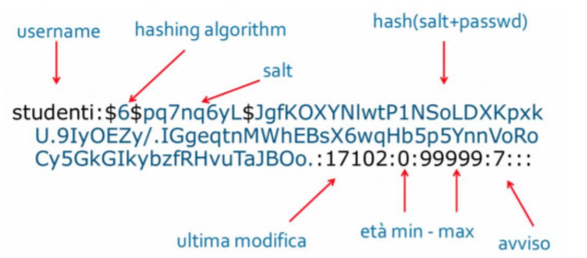
\includegraphics[scale=.9]{img/34.PNG}
			\end{center}
		\end{framed}
	\end{itemize}
	\item Attenzione alle variabili \emph{alfa} e \emph{beta}, che non solo sono presenti, ma anche globali (quindi vanno dichiarate).
	\begin{verbatim}
		.data
		alfa: .long 0
		beta: .long 0
	\end{verbatim}
	\item Chiamo la leggiint e sposto in \emph{alfa} il risultato, che sappiamo essere nel registro rax
	\begin{verbatim}
		call leggiint
		mov %eax, alfa(%rip)
	\end{verbatim}
	\item Stessa cosa con \emph{beta}
	\begin{verbatim}
		call leggiint
		mov %eax, beta(%rip)
	\end{verbatim}
	\item Metto in rdi il primo argomento e in rsi il secondo. Pongo inoltre il risultato in \emph{ris}
	\begin{verbatim}
		mov alfa(%rip), %edi
		mov beta(%rip), %esi
		call elab1
		mov %eax, -8(%rbp)
	\end{verbatim}
	\item Eseguo la scriviint ponendo \emph{ris} nel registro edi (secondo lo standard)
	\begin{verbatim}
		mov -8(%rbp), %edi
		CALL scriviint
	\end{verbatim}
	\item La funzione \emph{main} restituisce $0$ se tutto è andato per il verso giusto (un numero diverso da zero consiste nell'identificativo di un errore). Per restituire $0$ utilizziamo l'istruzione XOR sul registro EAX (RAX, bastano 32 bit visto che si restituisce un \emph{int})
	\begin{verbatim}
		xorl %eax, %eax
	\end{verbatim}
	\item Concludiamo sbarazzandoci del prologo e restituendo il controllo
	\begin{verbatim}
		leave
		ret
	\end{verbatim}
\end{itemize}
\paragraph{Osservazione} Possiamo includere in un file assembler servi.cpp?
\begin{verbatim}
	#include "servi.cpp"
\end{verbatim}
Il compilatore si lamenta (\emph{junk}). Non ha senso includere un file di un certo linguaggio in uno con un altro linguaggio. 
\paragraph{Ottimizzazione} 
L'ottimizzazione non si ottiene dalla riduzione del numero di istruzioni, ma da altre cose: scelta di istruzioni accurate, scritture in memoria solo quando necessario.

\subsubsection{Passaggio di parametri per riferimento (pag.41)}
Proviamo a fare una versione simile dell'esercizio precedente, ma con la presenza di un tipo di riferimento.
\begin{framed}
	\noindent \textbf{Codice c++}
	\begin{verbatim}
		// programma sommmaintRif, file es3a.cpp
		#include"servi.cpp"
		extern "C" void elab3(int& tot, int n1, int n2);
		int main() { 
			int a, b; int ris; <-------- a frosini e' sfuggita una &
			a = leggiint();
			b = leggiint();
			elab3(ris, a, b);
			scriviint(ris);
			nuovalinea();
		};
		// programma sommmaintRif, file es1b.cpp
		extern "C" int elab3(int& tot, int n1, int n2) { 
			int i, j;
			i = n1+n2;
			j = n1-n2;
			tot = i*j;
		};
	\end{verbatim}
\end{framed}
\paragraph{Traduzione Assembler di elab3}
\begin{verbatim}
	.text
	.global elab3
	elab3:
	push %rbp
	mov %rsp, %rbp
	sub $32, %rsp
	
	# copia tot al suo posto
	mov %rdi, -8(%rbp)
	
	# copia n1 ed n2 al suo posto
	mov %esi, -16(%rbp)
	mov %edx, -12(%rbp)
	
	# i = n1 + n2
	mov -16(%rbp), %eax
	add -12(%rbp), %eax
	mov %eax, -24(%rbp)
	
	# j = n1 - n2
	mov -16(%rbp), %eax
	add -12(%rbp), %ecx
	sub %eax, %ecx
	mov %ecx, -20(%rbp)
	
	# tot = i*j
	mov -24(%rbp), %eax
	imull -20(%rbp), %eax
	
	mov -8(%rbp), %rdx
	mov %eax, (%rdx)
	
	leave
	ret
\end{verbatim}

\begin{center}
	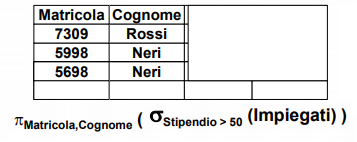
\includegraphics{img/35.PNG}
\end{center}
\begin{itemize}
	\item Pongo il vecchio rbp nella pila, aggiorno il valore di rbp e riservo 32 byte (32 invece di 24 per rispettare rsp multiplo di 16)
	\begin{verbatim}
		push %rbp
		mov %rsp, %rbp
		sub $32, %rsp
	\end{verbatim}
	\item Copio \emph{tot}, così come tutte le altre variabili (secondo lo standard) $n1$ ed $n2$.
	\begin{verbatim}
		mov %rdi, -8(%rbp)
		mov %esi, -16(%rbp)
		mov %edx, -12(%rbp)
	\end{verbatim}
	\item Sulla somma e sulla differenza non ci sono differenze importanti rispetto all'esercizio precedente.
	\item Recupero $i$ ponendolo in eax. Teniamo conto che in \&tot ci sarà l'indirizzo della variabile: sposto il contenuto della parte in un registro sporcabile, utilizzo l'indirizzamento indiretto per aggiornare il contenuto dell'indirizzo posto in rdx.
	\begin{verbatim}
		mov -24(%rbp), %eax
		imull -20(%rbp), %eax
		
		mov -8(%rbp), %rdx
		mov %eax, (%rdx)
	\end{verbatim}
	\item La funzione non restituisce niente, quindi mi limito a terminarla con \emph{leave} e \emph{ret}.
	\begin{verbatim}
		leave
		ret
	\end{verbatim}
\end{itemize}
\paragraph{Traduciamo anche il main}
\begin{verbatim}
	.text
	.global main
	main:
	push %rbp
	mov %rsp, %rbp
	
	call leggiint
	mov %eax, -8(%rbp)
	
	call leggiint
	mov %eax, -4(%rbp)   
	
	lea -16(%rbp), %rdi
	mov -8(%rbp), %esi
	mov -4(%rbp), %edx
	call elab3
	
	.Lnext:     
	mov -16(%rbp), %edi
	call scriviint
	call nuovalinea
	leave 
	ret
\end{verbatim}
\begin{center}
	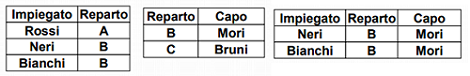
\includegraphics{img/36.PNG}
\end{center}
\begin{itemize}
	\item Pongo il vecchio rbp nella pila, aggiorno il valore di rbp e riservo un certo numero di byte per \emph{b}, \emph{a} e \emph{ris}.
	\item Le chiamate di leggiint non sono tanto diverse rispetto all'esercizio precedente
	\item Sposto nel registro rdi l'indirizzo della variabile \emph{tot} usando la LEA. Sistemo anche le variabili $n1$ e $n2$.
	\begin{verbatim}
		lea -16(%rbp), %rdi 
		mov -8(%rbp), %esi
		mov -4(%rbp), %edx
		call elab3
	\end{verbatim}
	\item Eseguo le funzioni rimanenti all'interno del \emph{main}, nulla di particolare da segnalare.
\end{itemize}
\subsubsection{Passaggio di parametro array (pag.50)}
\begin{framed}
	\noindent \textbf{Codice c++} 
	\begin{multicols}{2}
		\begin{verbatim}
			// programma array, file es6a.cpp
			#include "servi.cpp"
			extern "C" void raddoppia(int a[], int n);
			int main() {
				int ar[5];
				int i;
				for(i = 0; i < 5; i++)
				ar[i] = leggiint();
				raddoppia(ar, 5);
				for(i = 0; i < 5; i++)
				scriviint(ar[i]);
				nuovalinea();
			}
		\end{verbatim}
		\columnbreak
		\begin{verbatim}
			// programma array, file es6b.cpp
			extern "C" void raddoppia(int a[], int n){
				int i;
				for(i = 0; i < n; i++)
				a[i] = 2*a[i]; 
			}
		\end{verbatim}
	\end{multicols}
\end{framed}
\clearpage 
\paragraph{Traduzione assembler di raddoppia}
\begin{verbatim}
	.text
	.global raddoppia
	raddoppia: 
	push %rbp
	mov %rsp, %rbp
	sub $16, %rsp
	
	mov %rdi, -8(%rbp)
	mov %esi, -16(%rbp)
	
	# inizializzazione (i = 0)
	mov $0, -12(%rbp)
	.Lfor:     # Verifica della condizione (i < n)
	cmp %esi, -12(%rbp)
	jl .Lcorpo
	jmp .Lfine
	.Lcorpo:     
	# caricare %rdx
	movslq -12(%rbp), %rdx
	
	mov (%rdi, %rdx, 4), %eax
	sal $1, %eax <--- (stesso OPCODE di SHL)
	mov %eax, (%rdi, %rdx, 4)
	
	# i++
	incl -12(%rbp)
	jmp .Lfor
	.Lfine:      leave
	ret
\end{verbatim}

\begin{center}
	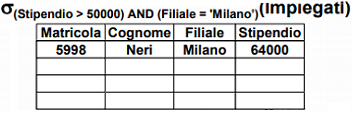
\includegraphics[scale=.9]{img/32.PNG}
\end{center} 
\begin{itemize}
	\item Pongo il vecchio rbp nella pila, aggiorno il valore di rbp e riservo un certo numero di byte per \emph{a}, \emph{n} ed \emph{i}.
	\begin{verbatim}
		push %rbp
		mov %rsp, %rbp
		sub $16, %rsp
	\end{verbatim}
	\item Pongo i valori degli argomenti in memoria
	\begin{verbatim}
		mov %rdi, -8(%rbp)
		mov %esi, -16(%rbp)
	\end{verbatim}
	per quanto riguarda l'array \emph{a} ricordiamoci che poniamo in memoria l'indirizzo del primo elemento dell'array. Ricordarsi che il primo elemento sta per forza negli indirizzi più bassi.
	\item Novità rispetto agli esercizi precedenti è l'introduzione di un for. Ricordiamo, a tal proposito, le spiegazioni sui cicli dalle dispense di Stea. In particolare, dobbiamo ricordare l'ordine delle operazioni in un for
	\begin{enumerate}
		\item inizializzazione del counter;
		\begin{verbatim}
			mov $0, -12(%rbp)
		\end{verbatim}
		\item verifica della validità della condizione;
		\item esecuzione del corpo del for (vedere dopo);
		\item ritorno al secondo punto.
		\begin{verbatim}
			jmp .Lfor
		\end{verbatim}
	\end{enumerate}
	\begin{framed}
		\item Dobbiamo caricare il registro rdx col valore del contatore, in modo da poterlo utilizzare per prendere l'elemento dell'array
		\begin{verbatim}
			movslq -12(%rbp), %rdx
		\end{verbatim}
		con questa istruzione teniamo conto del segno nel passaggio da \emph{long} a \emph{quad} (se utilizzo solo la MOV emergono problemi con un numero elevato di iterazioni). perché dobbiamo dire questo? \textbf{Nell'indirizzamento coi registri dobbiamo utilizzare registri a 64 bit} (il compilatore fa storie in caso contrario), tuttavia
		\begin{itemize}
			\item \textbf{il numero coinvolto nello spostamento è un numero a 32 bit},
			\item ed è anche intero.
		\end{itemize}
		Segue che \textbf{l'estensione di campo non è quella dei naturali} (in quel caso mi sarebbe bastato una semplice MOV con registri a 32 bit, considerato che i bit più significativi vengono azzerati)
	\end{framed}
	\item Sposto nel registro eax il valore da moltiplicare per due. Il prodotto è per una potenza della base due, quindi posso fare la cosa con uno shift a sinistra. Concludo riportando il numero shiftato in memoria.
	\begin{verbatim}
		mov (%rdi, %rdx, 4), %eax
		sal $1, %eax <--- va bene anche shl (stesso opcode)
		mov %eax, (%rdi, %rdx, 4)
	\end{verbatim}
	per quanto riguarda l'indirizzamento bimodificato
	\[\text{Indirizzo}=\left|\text{rdi}+\text{rdx}\times\text{4}\right|_{\text{modulo}_{2^{64}}}\]
	rdi è il registro avente per contenuto l'indirizzo del primo elemento dell'array (primo argomento della funzione), rdx è il registro dove poniamo ogni volta il contenuto della variabile contatore. Sapendo che ogni intero occupa 4 byte si capisce al volo che incrementando rdx passeremo all'elemento immediatamente successivo dell'array.
\end{itemize}
\paragraph{Traduciamo anche il main}
\begin{verbatim}
	.set ar, -24
	.set i, -32
	
	.text
	.global main
	main:
	push %rbp
	mov %rsp, %rbp
	sub $32, %rsp
	
	movl $0, i(%rbp) # <---- i = 0
	.Lfor1:        cmp $5, i(%rbp), 
	jl .Lcorpo1 # <--- i < 5
	jmp .Lfine1
	.Lcorpo1:
	call leggiint
	movslq i(%rbp), %rcx
	mov %eax, ar(%rbp, %rcx, 4)
	incl i(%rbp)
	jmp .Lfor1 # ritorno alla condizione 
	.Lfine1:       lea -24(%rbp), %rdi
	mov $5, %esi
	call raddoppia
	
	movl $0, i(%rbp)
	.Lfor2:
	cmp $5, i(%rbp)
	jl .Lcorpo2
	jmp .Lfine2
	.Lcorpo2:
	movslq i(%rbp), %rcx
	mov ar(%rbp, %rcx, 4), %rdi
	call scriviint
	incl i(%rbp)
	jmp .Lfor2
	.Lfine2:
	call nuovalinea
	
	leave
	ret
\end{verbatim}
\begin{center}
	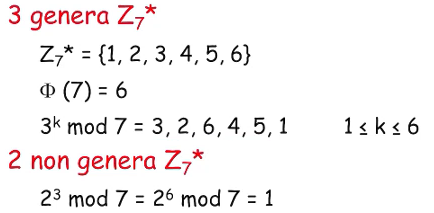
\includegraphics[scale=.9]{img/23.PNG}
\end{center} 
\begin{itemize}
	\item Nella creazione dell'array trattiamo ogni elemento come se fosse un qualcosa di indipendente. Li poniamo in modo tale che l'allineamento sia rispettato. Un modo per ricordarsi che l'array deve essere posto in un certo modo sono le istruzioni per visitare, in un ciclo, tutti gli elementi dell'array (somma sul puntatore ad array): se poniamo in fondo alla pila (negli indirizzi più alti) il primo elemento allora il meccanismo non funziona.
	\begin{framed}
		\item \textbf{Direttive \emph{set}}. Con le direttive \emph{set} andiamo a creare delle costanti (già visto a Reti logiche, ricordarsi \emph{pippo} e la domanda del pretest).
		\begin{verbatim}
			.set ar, -24
			.set i, -32
		\end{verbatim} Possiamo assegnare SOLO delle costanti, non stiamo lavorando con delle macro. 
		\begin{verbatim}
			.set i, -32(%rbp) <------- SBAGLIATO!
		\end{verbatim}
	\end{framed}
	\item Come al solito memorizziamo il vecchio rbp e allochiamo lo spazio necessario
	\begin{verbatim}
		push %rbp
		mov %rsp, %rbp
		sub $32, %rsp
	\end{verbatim}
	\item Poniamo in rdi l'indirizzo dell'array, che è l'indirizzo del primo elemento dell'array.
	\begin{verbatim}
		lea -24(%rbp), %rdi
	\end{verbatim}
	non si utilizzi la mov invece della lea
	\begin{verbatim}
		mov -24(%rbp), %rdi
	\end{verbatim}
	che sposta in memoria il contenuto del primo elemento dell'array, E NON L'INDIRIZZO DELLO STESSO!
	\item Poniamo anche il secondo argomento e chiamiamo la funzione \emph{raddoppia}
	\begin{verbatim}
		mov $5, %esi
		call raddoppia
	\end{verbatim}
	\item Il for per la stampa dell'array (legata alla funzione \emph{scriviint}) non è strutturato in modo diverso dal primo.
	\begin{framed}
		\item \textbf{Osservazione sui registri \emph{scratch}}: Uno studente si è accorto di un errore del prof nell'uso del registro rcx. Il codice inizialmente era così
		\begin{verbatim}
			movslq i(%rbp), %rcx
			call leggiint
			mov %eax, ar(%rbp, %rcx, 4)
		\end{verbatim}
		La cosa è un problema: rcx, essendo scratch, potrebbe non essere preservato nella funzione \emph{leggiint}. Se proviamo ad eseguire otterremo un \emph{Bus error}: questo perché la modifica dell'rcx da parte di \emph{leggiint} ci porta nel cosiddetto \emph{buco della memoria} (la parte di memoria non utilizzata introdotta nelle lezioni precedenti). Abbiamo due soluzioni possibili:
		\begin{itemize}
			\item scegliere un registro \emph{non scratch}
			\item invertire le prime due righe della parte incriminata (soluzione adottata dal prof per questo caso)
		\end{itemize}
	\end{framed}
\end{itemize}

\subsubsection{Passaggio di parametro struttura (pag.64)}
\begin{framed}
	\noindent \textbf{Codice c++} 
	\begin{multicols}{2}
		\begin{verbatim}
			// programma struttura, file es10a.cpp
			#include "servi.cpp"
			struct s  { int n1; char c; int n2; };
			extern "C" s leggis() {
				s ss;
				ss.n1 = leggiint();
				ss.c = leggichar();
				ss.n2 = leggiint();
				return ss; 
			}
			extern "C" void scrivis(s ss) {
				scriviint(ss.n1);
				scrivichar(ss.c);
				scriviint(ss.n2);
				nuovalinea();
			}
			
			extern "C" s fai(s st);
			int main() {
				s st1, st2;
				st1 = leggis();
				st2 = fai(st1);
				scrivis(st2);
				return 0;
			}
			
			// programma struttura, file es10b.cpp
			struct s { int n1; char c; int n2; };
			extern "C" s fai(s st) {
				s ss;
				ss.n1 = st.n1 + 5;
				ss.c = st.c + 1;
				ss.n2 = st.n2 + 10;
				return ss;
			}
		\end{verbatim}
	\end{multicols}
\end{framed}

\noindent \textbf{Traduzione assembler di es10b}
\begin{verbatim}
	.text
	.global fai
	fai:
	push %rbp
	mov %rsp, %rbp
	sub $32, %rsp
	mov %rdi, -16(%rbp)
	mov %esi, -8(%rbp)
	
	# ss.n1 = st.n1 + 5
	mov -16(%rbp), %eax
	add $5, %eax
	mov %eax, -32(%rbp)
	# ss.c = st.c + 1
	mov -12(%rbp), %al
	add $1, %al
	mov %al, -28(%rbp)
	# ss.n2 = st.n1 + 10
	mov -8(%rbp), %eax
	add $10, %eax
	mov %eax, -24(%rbp)
	# return ss
	mov -32(%rbp), %rax
	mov -24(%rbp), %edx
	
	leave
	ret
\end{verbatim}
\begin{center}
	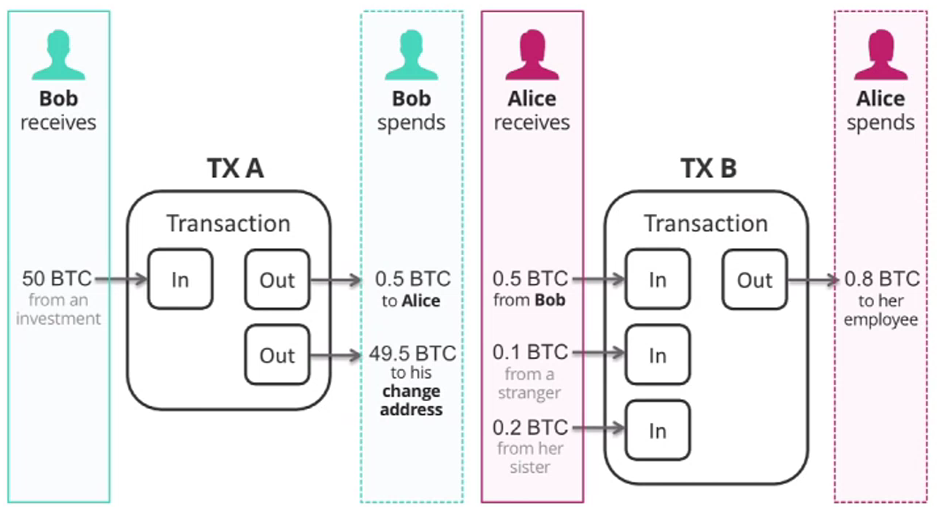
\includegraphics[scale=.9]{img/31.PNG}
\end{center} 
\begin{itemize}
	\item Nel riservare lo spazio agli elementi della struttura ricordiamo lo stesso ragionamento visto per gli array: se io incremento devo passare all'elemento successivo. Segue che \textbf{in cima alla pila (indirizzi più bassi) ci saranno i primi elementi della struttura}.
	
	\item Memorizziamo l'rbp vecchio e riserviamo lo spazio di memoria necessario, in luce delle considerazioni precedenti
	\begin{verbatim}
		push %rbp
		mov %rsp, %rbp
		sub $32, %rsp
	\end{verbatim}
	\item Sistemiamo la struttura posta in ingresso come parametro. Abbiamo 16byte divisi in due blocchi, seguono due operazioni di mov. Si consideri che finchè il parametro sta in 16byte non è un problema. Segue
	\begin{verbatim}
		mov %rdi, -16(%rbp)
		mov %esi, -8(%rbp)
	\end{verbatim}
	\textbf{Nel primo registro vanno i primi elementi della struttura, i rimanenti nel secondo registro.}
	\item Per le operazioni di somma
	\begin{itemize}
		\item spostiamo l'operando non costante dalla memoria a un registro
		\item eseguiamo l'addizione su quel registro
		\item spostiamo il contenuto modificato nella variabile indicata nell'assegnamento
	\end{itemize}
	segue
	\small
	\begin{verbatim}
		# ss.n1 = st.n1 + 5
		mov -16(%rbp), %eax # <------------ sposto st.n1 in eax
		add $5, %eax # <----- sommo 5 ad eax
		mov %eax, -32(%rbp) # <--- sposto il contenuto addizionato in ss.n1
		
		# ss.c = st.c + 1
		mov -12(%rbp), %al # <---- sposto st.c in al
		add $1, %al # <------- sommo 1 ad al
		mov %al, -28(%rbp) # <---- sposto il contenuto incrementato in ss.c
		
		# ss.n2 = st.n1 + 10
		mov -8(%rbp), %eax # <---- sposto st.n1 in eax
		add $10, %eax # <----- sommo 10 ad eax
		mov %eax, -24(%rbp) # <----- sposto il contenuto addizionato in ss.n2
	\end{verbatim}
	\item La struttura è di 16byte, divisa in due blocchi. Dobbiamo eseguire due spostamenti di memoria per la struttura restituita dalla funzione 
	\begin{verbatim}
		mov -32(%rbp), %rax
		mov -24(%rbp), %edx
	\end{verbatim}
	Come parte meno significativa poniamo la prima riga della struttura (quella a indirizzo più basso, col primo intero e il char), l'altra come parte più significativa (quella col secondo intero).
	\item Chiudiamo come al solito
	\begin{verbatim}
		leave
		ret
	\end{verbatim}
	\begin{framed}
		\item \textbf{Osservazione sulla dichiarazione delle strutture}.
		\begin{verbatim}
			struct s  { int n1; char c; int n2; };
		\end{verbatim}
		Ricordiamoci che il compilatore lavora singolarmente su ogni file. 
		\begin{itemize}
			\item Nel file col main abbiamo la dichiarazione della struttura \emph{s} (la utilizziamo nel main, è fondamentale perché il compilatore deve sapere quanto spazio allocare per la struttura - non tanto per gli elementi interni)
			\item Nel file con la funzione \emph{fai} si potrebbe pensare che non è necessario definire la struttura \emph{s}: FALSO, altrimenti il compilatore non potrà conoscere gli offset della struttura (la funzione \emph{fai} lavora su singoli elementi delle strutture)
		\end{itemize}
	\end{framed}
	\item \textbf{Proviamo a cambiare la struttura \emph{s} in uno dei due files: se ne accorge qualcuno?}
	
	Il compilatore no, visto che lavora sui singoli files. Il collegatore vede tutto insieme, ma non si preoccupa di queste cose. Quindi, se siamo fortunati, non se ne accorge nessuno. Se modifico la definizione nel primo file non è un problema: sposto gli elementi ma la dimensione complessiva della struttura è la stessa. Nel secondo file, invece, la cosa genera problemi: non vengono segnalati errori, ma il risultato ottenuto non è quello desiderato.
\end{itemize}
\paragraph{Traduzione assembler del main}
\begin{center}
	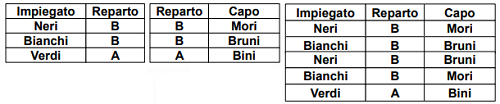
\includegraphics{img/37.PNG}
\end{center} 
\begin{verbatim}
	.text
	.global main
	main:
	push %rbp
	mov %rsp, %rbp
	
	call leggis
	mov %rax, -16(%rbp)
	mov %edx, -8(%rbp) # <---- memorizzo la struttura restituita in st1
	
	mov -16(%rbp), %rdi
	mov -8(%rbp), %edx # <--- pongo la struttura st1 come argomento della funzione fai
	call fai
	mov %rax, -32(%rbp)
	mov %edx, -24(%rbp) # <--- memorizzo la struttura restituita in st2
	
	mov -32(%rbp), %rdi
	mov -24(%rbp), %esi # <--- pongo la struttura st2 come argomento della funzione scrivis
	call scrivis
	
	xorl %eax, %eax # <--- restituisco 0
	leave
	ret # <---- concludo come al solito
\end{verbatim}
\endgroup